\chapter{Single-Machine Implementations}\label{sec-implement}
In this chapter, we present the implementation details of Mars on a
single machine. The current Mars system consists of four modules
(Table \ref{tb:impls}). All these four modules share the common
design of Mars, and provide the same MapReduce interface to the
user. They can run on different hardware platforms: MarsCUDA on
an NVIDIA GPU, MarsBrook on an AMD GPU, MarsCPU on a multi-core CPU,
and the GPU/CPU co-processing module on both the CPU and the GPU
through combining the aforementioned modules.  Different modules in
Mars allow programmers to take advantage of different processors on
a single machine. Because our machines cannot host a multi-GPU configuration due to limited extension slots, we have not explored multi-GPU co-processing.

\begin{table}[htb]
  \centering
 \linespread{1.7}{ {\footnotesize
  \caption{Modules in the Mars system}\label{tb:impls}
\vspace{2em}
  \begin{tabular}{ccc}
  \hline
\noalign{\smallskip}
  \textbf{Implementation} & \textbf{Software platform} & \textbf{Hardware platform}\\
\noalign{\smallskip}
  \hline
  MarsCUDA & NVIDIA CUDA & an NVIDIA GPU \\
  MarsBrook & AMD Brook+ & an AMD GPU \\
  MarsCPU & pthreads & a multi-core CPU \\
  GPU/CPU co-processing & CUDA/Brook+ and pthreads &  NVIDIA/AMD GPUs and multi-core CPUs\\
\noalign{\smallskip}
  \hline
  \end{tabular}
  }}
\end{table}

\section{MarsCUDA}

We implemented MarsCUDA using NVIDIA CUDA. We used the GPU
Prefix Sum routine from CUDPP~\cite{CUDPP} to implement the lock-free scheme, and
the GPU Bitonic Sort routine for the {\em Group} phase.
CUDA exposes sufficient hardware details of NVIDIA GPUs, so that we can
apply some optimizations in MarsCUDA runtime.
\\\\
{\em 1. Memory access}
\\
{\bf Coalesced access.} We utilize the NVIDIA GPU feature of
coalesced access to improve the memory performance. In CUDA,
simultaneous device memory accesses by threads in a half-warp (warp is an NVIDIA term for a group of 32 threads for scheduling) can be
coalesced into a single memory transaction, which significantly
reduces the number of device memory accesses.
We implement the access to the directory index arrays as coalesced.

\red{{\bf Local  memory.} NVIDIA  GPUs  provide  the programmable  on-chip  local  memory  (or \emph{shared memory}~\cite{CUDA2008}), for sharing data among threads running on the same multiprocessor. It is important to fully utilize the local memory to reduce the costly accesses to the GPU memory. In Mars, data sharing or communication only happens in the Group stage. MarsCUDA runtime automatically uses a GPU-based bitonic sort~\cite{He2008} to exploit this memory hierarchy in the Group stage. Mars does not expose the local memory to the user-defined functions in the Map and the Reduce stages. Since local memory is programmer-controlled fast memory, it introduces complexity and needs the effort from the programmer. This is a trade-off between performance and programmability.  Nevertheless, users who are aware of the GPU memory hierarchy and need such data sharing can exploit the local memory in implementing the Map (or Reduce) function.
}
%{\bf Local memory.} NVIDIA GPUs provide programmable on-chip local memory (or shared memory in CUDA term), for sharing data among threads running on the same multiprocessor.  It is critical to well utilize local memory to achieve high GPU memory bandwidth.  In MapReduce framework, data sharing or communication only happens between the Map stage and the Reduce stage, that is, the Group stage in Mars.  MarsCUDA runtime automatically exploits this memory hierarchy in the Group stage, which is a GPU-based bitonic sort.  During the Map (or Reduce) stage, each Map (or Reduce) task is independent, and there is little opportunity for data sharing between the tasks.  Moreover, since local memory must be programmed explicitly, it introduces complexity and needs the effort from the programmer. This is a trade-off between performance and programmability.  Nevertheless, users who are aware of the GPU memory hierarchy and need such data sharing can exploit the local memory in implementing the Map (or Reduce) function.

\red{
{\bf Built-in vector types.}
%Accessing data values in the device memory can be costly, because they are often of different sizes and the accesses are hardly coalesced.  Fortunately, GPUs support built-in vector types \cite{CUDA2008}, including {\em char4} and {\em int4}.
Data accesses in the GPU device memory should be aligned to make sure the correctness and achieve high memory bandwidth.
Fortunately, GPUs support built-in vector types \cite{CUDA2008}, including {\em float4} and {\em int4}.
The alignment requirement is automatically fulfilled for built-in types.
%A read of a built-in vector fetches the entire vector in a single memory request.
In addition, the GPU is able to issue a single load instruction to read data of built-in type, of size up to 16 bytes.
%Compared with reading {\em char} or {\em int}, the number of memory requests in reading {\em char4} or {\em int4} is greatly reduced and the memory performance is improved.
Compared with reading an array one {\em float} or {\em int} at a time, the number of compiler-generated instructions for reading {\em float4} or {\em int4} is greatly reduced and the overall performance is improved.
}

\red{
{\bf Page-locked host memory.} CUDA supports page-locked host memory (a.k.a pinned), which prevents the operating system from paging the locked memory buffer, yielding high transfer bandwidth between the device memory and the host memory \cite{CUDA2008}.
The MarsCUDA runtime utilizes the page-locked host memory mechanism, in order to reduce the data transfer overhead. Our test demonstrated that page-locked memory can double the memory transfer rate through PCI-E bus than pageable memory.}
\\\\
{\em 2. Parallelism}
\\
Since CUDA exposes the thread configuration, we utilize the parallelism by assigning the tasks to
a large number of threads. The thread configuration, i.e., the number of thread blocks and the
number of threads per thread block, is related to both hardware and software factors:
 (1) the hardware configuration such as the number of
multiprocessors and the on-chip computation resources such as the
number of registers on each multiprocessor, and (2) the characteristics of the map and the reduce tasks, e.g., the degree of memory- or computation-intensiveness.

Since the map and the reduce functions are implemented by the
developer, and their costs are unknown to the runtime system, it is
difficult to find the optimal setting for the thread configuration
at run time. CUDA provides an off-line
calculator~\footnote{http://developer.download.nvidia.com/compute/cuda/CUDA\_Occupancy\_calculator.xls}
for computing the multiprocessor occupancy given a CUDA program. For
the program (either the map task or the reduce task), the calculator
takes the number of threads per thread block and the number of
registers used per thread as input, and outputs the occupancy and
the number of active thread blocks per multiprocessor. The number of
registers used per thread is obtained using the NVCC compiler of
CUDA.

With the calculator, we iterate the number of threads per block in
multiples of 32 (the schedule unit size) ranging from 32 to 512 (the
maximum number of threads per thread block), until the occupancy is
higher than a predefined threshold. Thus, we get the number of
threads per thread block and the number of thread blocks. In
practice, we set the occupancy threshold to be 2/3 so that the GPU
is sufficiently busy, and each thread block receives adequate
computation resources.


%We determine the thread configuration according to the warp occupancy on the multiprocessor.
%The thread configuration includes the number of threads per thread group $N_{t}$,
%and the number of thread groups $N_{g}$.
%Multiple factors determine the thread configuration, including
%the hardware configuration such as the number of multiprocessors and
%the on-chip computation resources such as the number of registers on each multiprocessor
%and the usage of on-chip local memory (shared memory).


%Since the map and the reduce functions are implemented by the developer, and their costs are unknown to the runtime system,
%it is difficult to find the optimal setting for the thread configuration at run time.
%Fortunately, CUDA provides an off-line calculator for computing the multiprocessor warp occupancy given a CUDA program,
%and then determine $N_{t}$.
%For the program (either the map task or the reduce task), the calculator takes the number of threads per thread group $N_{t}$,
%the number of registers used per thread and the usage of local memory per block as input,
%and outputs the occupancy, which is the number of active warps per multiprocessor.
%The number of registers used per thread and the usage of local memory per block are obtained using the NVCC compiler of CUDA.
%With the calculator, we iterate the number of threads per group in multiples of 32 (the schedule unit size) ranging from 32 to 512
%(the maximum number of threads per thread group), until the occupancy is higher than a predefined threshold.
%Thus, we get the number of threads per thread group $N_{t}$.
%In practice, we set the occupancy threshold to be 2/3 so that the GPU is sufficiently busy,
%and each thread group receives adequate computation resources.
%
%
%We obtain the number of threads per thread group $N_{t}$ manually,
%and obtain the number of thread groups $N_{g}$ automatically during the runtime.
%For the Map stage, given the number of input records $N_{r}$, we get:
%\begin{center}
%$N_{g} = \lceil \frac{N_{r}}{N_{t} \times num\_rec\_map} \rceil$
%\end{center}
%$num\_rec\_map$ is the parameter configured by users, meaning the number of records processed per map task.
%It is similar for the Reduce stage, so we skip that.

\section{MarsBrook} \label{sec-brook}
We implement MarsBrook on AMD GPUs using the stream programming
model Brook+ \cite{BROOKPLUS}.
Due to the limitation of Brook+, MarsBrook is less advanced than MarsCUDA in both expressivity and performance.
Nevertheless, as programming support of Brook+ improves, MarsBrook can demonstrate a higher flexibility and performance.

MarsBrook requires users to specify the data types of keys and values statically, and each record is of a fixed size.
Type conversion is not allowed in Brook+. Unlike CUDA, Brook+ does not allow the developer to access data in GPU memory by arbitrary address.
Instead, data in the GPU memory is accessed using a {\em stream}, which is essentially a sequentially-accessed array of fixed-sized elements. Random access in a stream is achieved by providing another predefined stream, consisting of indexes of target elements to access.
\red{Although the Mars APIs are the same on CUDA and on Brook+, as listed in Table \ref{tb:marsapi},
using Mars on CUDA is more flexible than using that on Brook+ when the Mars user develops a user-defined function.
}

Moreover, MarsBrook has relatively limited room for performance optimization.
The reason is that Brook+ does not expose detailed hardware
features, e.g., fast on-chip local memory, coalesced memory access,
or GPU thread configuration.



%While the implementation of MarsBrook shows the general design of
%Mars is also feasible to AMD GPUs, other than NVIDIA GPUs.

\section{MarsCPU}
We implement MarsCPU using the pthreads library on linux for multi-threading.
Instead of adopting lock-based task scheduling as in Phoenix,
MarsCPU inherits the lock-free design of GPU-based Mars, which we expect to scale to hundreds of cores for future many-core CPUs.
MarsCPU deploys CPU threads to perform Map and Reduce tasks.
If there are $N$ Map (or Reduce) tasks, and $T$ CPU threads, where $N$ is usually much larger than $T$, then a thread processes $\lceil N/T \rceil$ tasks.
We implement a CPU multi-threaded parallel mergesort for the Group stage.

\section{GPU/CPU co-processing} \label{sec-coprocessing}

%Since both the CPU and the GPU are integrated components on a
%commodity machine, we develop MapReduce with co-processing on these
%two kinds of processors to fully utilize their computation power.

The workflow of GPU/CPU co-processing is shown in Figure \ref{fig:Mars+}.
There are also mainly three stages, {\em Map}, {\em Group} and {\em Reduce}.
In the {\em Map} stage,
the scheduler divides the input data into multiple chunks. The
number of chunks is equal to the total number of CPUs and GPUs in
the machine. The chunk sizes are determined based on the performance
comparison between the CPU and the GPU. Suppose the speedup of the
GPU worker over the CPU worker is $S$, where the {\em speedup} is
defined to be the ratio of the execution time on the CPU to that on
the GPU for the same amount of input data. Given the total input
size of $I$ bytes, we assign data chunks of $\frac{SI}{1+S}$ and
$\frac{I}{1+S}$ bytes to the GPU and the CPU workers, respectively.
\red{The speedup $S$ can be obtained by either calibration or predictive model \cite{Kerr2010}.}

When a processor finishes a {\em Map} task, it performs a local {\em Group} on intermediate results.
The runtime merges all intermediate results. When all the processors finish their
tasks, the {\em Map} stage ends.

The {\em Reduce} stage takes the intermediate results from the {\em Group} stage
as input. Similar to the {\em Map} stage, the co-processing scheduler statically assigns the
data chunks to the processors. When all the processors finish their
tasks, the runtime merges all local results.

%Please note that, workload dispatching between the GPU worker and the CPU worker by speedup works well only under two conditions.
\red{
Mars dispatches workload between the GPU worker and the CPU worker only if the following conditions are satisfied.
First, the Map and Reduce stages take up high proportion of the entire running time on the CPU worker. If components other than the Map and Reduce stages contribute to a large portion of running time, the GPU worker is not able to make large performance acceleration. Second, the GPU worker and the CPU worker have comparable performance. The benefit of using the CPU worker diminishes, as the speedup of the GPU worker over the CPU worker becomes higher. 
}
\begin{figure}[h]
  \centering
  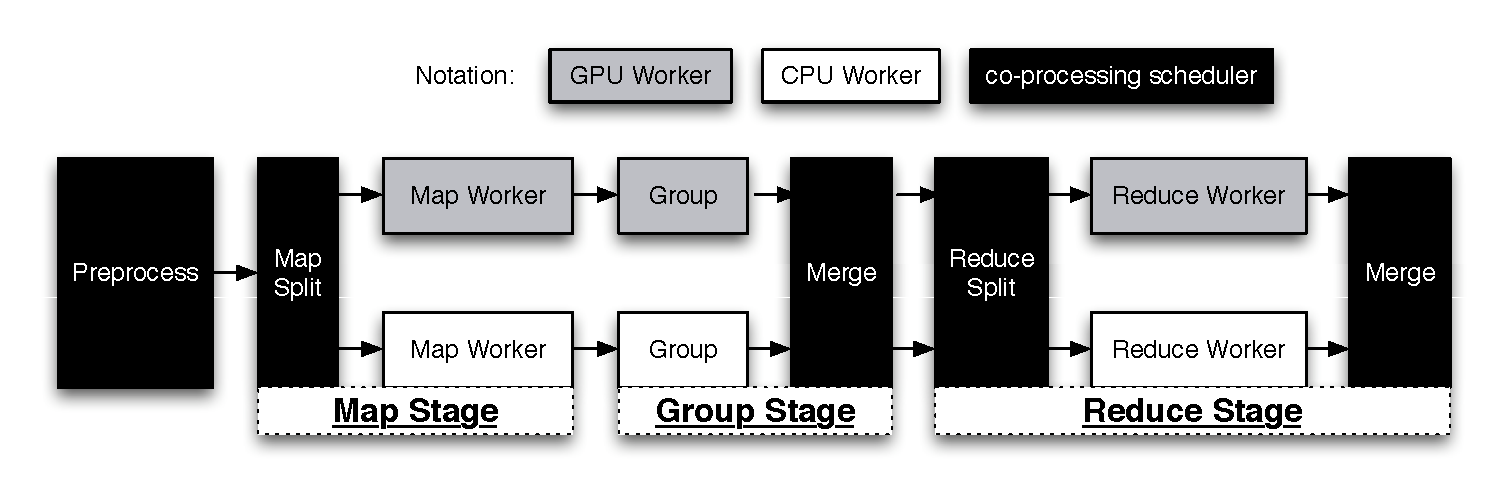
\includegraphics[width=1.00\textwidth]{figure/Mars+.eps} 
  \caption{The workflow of GPU/CPU co-processing. }\label{fig:Mars+}
\end{figure}

With the GPU/CPU co-processing module, Mars can harness the
computation power of NVIDIA GPUs, AMD GPUs, and multi-core CPUs on
the same machine, by integrating MarsCUDA, MarsBrook, and MarsCPU
modules as components.
